\documentclass[11pt,a4paper]{ctexart}
\usepackage{amssymb,amsmath}
\usepackage{graphicx}
\usepackage{enumerate}
\usepackage{listings}
\usepackage{color}
\usepackage{pgfplots}

% 设置版面参数
\setlength{\textwidth}{162mm}
\setlength{\textheight}{231mm}
\setlength{\headheight}{0cm}
\setlength{\topmargin}{-0.1cm}
\setlength{\oddsidemargin}{0cm}
\setlength{\evensidemargin}{0cm}
\setlength{\parskip}{1mm}
\setlength{\unitlength}{1mm}
\setlength{\parindent}{2.06em}

\begin{document}
\lstset{language=TeX}

\title{\LaTeX 入门:\\
  {\large 学习排版科技类文档}}
\author{桂义林\thanks{Email: yilin.gui@gmail.com}}
\date{\today}
\maketitle

\begin{abstract}
\LaTeX 是专为学术、科技写作开发的语言和程序,拥有强大的package支持,使用\LaTeX 写作可以避免使用Word带来的一些令人头疼的排版问题,如手动调整页边距、引用格式之类。本文旨在简单介绍\LaTeX 入门级别的使用方法,使不了解\LaTeX 的人阅读后能够利用\LaTeX 进行简单的科技类文档写作。本文的内容包括:\LaTeX 排版命令基础、数学公式排版、表格与插图、使用BibTeX 管理文献和Beamer包制作演示文稿简介。
\end{abstract}

\section{\LaTeX 的安装}
\subsection{\LaTeX 发行版}
一般选择直接安装\LaTeX 发行版,常见的有跨平台的TeX Live,Windows下的MikTeX、CTeX,Mac OS X 下的MacTeX。Linux下推荐安装TeX Live(http://tug.org/texlive/),最新版本为TeX Live 2014。

\subsection{关于中文支持}
如果使用Windows下的CTeX,使用其集成的CJK宏包可以方便地支持中文。但在Linux下使用\LaTeX 需要对中文支持进行额外的配置,一般可以选择使用CTeX宏包与xeCJK宏包组合。具体配置方法不在本文的讨论范围之内,请自行搜索互联网解决。

\subsection{线上编辑\LaTeX 文档}
www.sharelatex.com 和www.writelatex.com 这两个网站提供了线上编辑\LaTeX 文档的功能,可以自动保存工作进度,并支持多人协作。


\section{\LaTeX 排版命令基础}
\subsection{\LaTeX 文档结构}
先看一个典型的文档头声明:
\begin{lstlisting}[frame=single]
\documentclass[a4paper]{article}
\usepackage{amssymb,amsmath}
\usepackage{graphicx}
\end{lstlisting}

上面代码的第一行表明文档类型为一般期刊文章,下面两行是宏包的引用。

\LaTeX 命令的基本形式为:
\begin{lstlisting}[frame=single]
\command[options]{arguments}
\end{lstlisting}

一篇完整文档的结构示例如下:
\begin{lstlisting}[frame=single]
\documentclass[a4paper]{article}
\usepackage{amssymb,amsmath}
\usepackage{graphicx}

\begin{document}

\end{document}
\end{lstlisting}

文档类型包括但不限于:
\begin{itemize}
\item article:一般的期刊文章
\item book: 书籍
\item report: 研究报告
\end{itemize}

\subsection{字体、字号相关}
\LaTeX 中通过命令对字体、字号、文字颜色等进行控制,并通过预定义的命令生成希腊字母等特殊符号。

下面看一个例子:
\begin{lstlisting}[frame=single]
{\normalsize normal size text}\\
{\huge big size text}\\
{\color{red} red text}\\
\textbf{bold text}
\end{lstlisting}

上面代码的输出结果为:\\
{\normalsize normal size text}\\
{\huge big size text}\\
{\color{red} red text}\\
\textbf{bold text}

\begin{figure}[htbp]
\centering
\includegraphics[width=12cm]{latex_fontsize.pdf}
\caption{\LaTeX 中的字号} \label{fig:latex_font_size}
\end{figure}

\begin{figure}[htbp]
\centering
\includegraphics[width=12cm]{latex_symb.pdf}
\caption{\LaTeX 特殊符号:希腊字母} \label{fig:latex_symb}
\end{figure}

\subsection{章节环境}

常用的章节环境有:
\begin{itemize}
\item part
\item chapter
\item section
\item subsection
\end{itemize}

使用章节环境会生成相应章节标题,帮助我们确定文章的逻辑结构。

用法:
\begin{lstlisting}[frame=single]
\section{Introduction}

\section{Developing a Morphing Program}
\subsection{The Morphing Process}
\subsection{The User Interface}
\end{lstlisting}

\subsection{其他排版命令}
\LaTeX 排版命令有很多,不要期望一下记住所有命令的使用方法,应该在使用中学习和积累。下面再介绍一些常用的命令。

条目列表:

\begin{lstlisting}[frame=single]
\begin{itemize}
\item apple
\item banana
\item cherry
\end{itemize}
\end{lstlisting}

\begin{itemize}
\item apple
\item banana
\item cherry
\end{itemize}

枚举列表:

\begin{lstlisting}[frame=single]
\begin{enumerate}
\item apple
\item banana
\item cherry
\end{enumerate}
\end{lstlisting}

\begin{enumerate}
\item apple
\item banana
\item cherry
\end{enumerate}

使用$\backslash$title、$\backslash$author声明标题和作者,使用$\backslash$maketitle生成标题和作者。

\section{数学公式排版}
\TeX 的发明就是为了解决数学公式的排版,\LaTeX 是目前公认的对数学公式排版最强的系统。

\LaTeX 中的公式分为行间公式和行内公式,行间公式单独成行,行内公式就是在文字行内的公式。

行内公式示例:
\begin{lstlisting}[frame=single]
Euler's formula: $e^{ix}=\cos{x}+i\sin{x}$.
Not very complex:
\begin{math}
\Gamma_{ij}^{k}
=\frac{1}{2}(\frac{\partial g_{il}}{\partial u^j}
+\frac{\partial g_{jl}}{\partial u^i}
-\frac{\partial g_{ij}}{\partial u^l})
\end{math}
\end{lstlisting}

Euler's formula: $e^{ix}=\cos{x}+i\sin{x}$.
Not very complex:
\begin{math}
\Gamma_{ij}^{k}
=\frac{1}{2}(\frac{\partial g_{il}}{\partial u^j}
+\frac{\partial g_{jl}}{\partial u^i}
-\frac{\partial g_{ij}}{\partial u^l})
\end{math}
\vspace{1cm}

行间公式示例:

\begin{lstlisting}[frame=single]
\[\iiint_{\Omega}f(x,y,z)dxdydz \]
\begin{equation}
\left|\begin{array}{cccc}
1 & 6 & 9 \\
7 & 90 & f(x)\\
9 & \psi(x) & g(x)
\end{array}\right|
\end{equation}
\end{lstlisting}

\[\iiint_{\Omega}f(x,y,z)dxdydz \]
\begin{equation}
\left|\begin{array}{cccc}
1 & 6 & 9 \\
7 & 90 & f(x)\\
9 & \psi(x) & g(x)
\end{array}\right|
\end{equation}
\vspace{0.2cm}

使用\LaTeX 生成的数学公式就是如此简洁、高效!目前一些论坛、博客也支持\LaTeX 格式的数学公式输入,使得互联网上对数学问题的讨论、交流更加方便。

\section{表格与插图}
\subsection{生成表格}
使用 tabular 环境可以生成表格,我们来看一个例子:
\begin{lstlisting}[frame=single]
\begin{table}[hbtp]
\caption{This table is an example}
\begin{center}
\begin{tabular}{c|cc}
First row, first column &
  First row, second column &
  First row, third column \\ \hline
Second row, first column &
  Second row, second column &
  Second row, third column \\
Third row, first column &
  Third row, second column &
  Third row, third column \\
\multicolumn{3}{c}{...}
\end{tabular}
\end{center}
\end{table}
\end{lstlisting}

\begin{table}[hbtp]
\caption{This table is an example}
\begin{center}
\begin{tabular}{c|cc}
First row, first column &
  First row, second column &
  First row, third column \\ \hline
Second row, first column &
  Second row, second column &
  Second row, third column \\
Third row, first column &
  Third row, second column &
  Third row, third column \\
\multicolumn{3}{c}{...}
\end{tabular}
\end{center}
\end{table}

\clearpage

\subsection{插入图形}
可以使用graphicx宏包支持图形的插入,在文档头部加入$\backslash$usepackage\{graphicx\},在需要插图的地方使用$\backslash$includegraphics命令。

需要注意\LaTeX 本身仅支持eps(矢量图形格式)和pdf两种格式的图片(使用LaTeX命令编译),使用PDFLaTeX 编译可以支持png 和jpg 格式的图片。一般来说正式的论文中是不允许使用jpg或png 格式的图片的。

例子:

\begin{lstlisting}[frame=single]
\begin{figure}[hbtp]
\begin{center}
\includegraphics[scale=0.3]{TUGlog.pdf}
\end{center}
\caption{TeX User Group Logo}
\end{figure}
\end{lstlisting}

\begin{figure}[hbtp]
\begin{center}
\includegraphics[scale=0.3]{TUGlog.pdf}
\end{center}
\caption{TeX User Group Logo}
\end{figure}
\vspace{0.5cm}

值得一提的是,\LaTeX 本身拥有绘图工具包(pgfplots),因此不借助第三方工具仅仅靠\LaTeX 生成高质量的论文插图也是可行的!

下面看一个pgfplots绘图的例子:

\begin{lstlisting}[frame=single]
\begin{figure}[hbtp]
\begin{center}
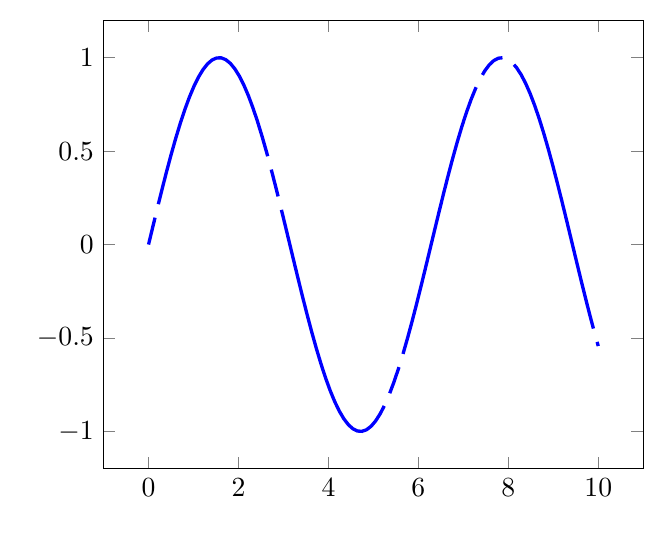
\begin{tikzpicture}
\begin{axis}
\addplot [dash pattern=on 10 off 5 on 100 off 5,
  domain=0:10, samples=100, very thick, blue] {sin(deg(x))};
\end{axis}
\end{tikzpicture}
\end{center}
\caption{This is generated by pgfplots!}
\end{figure}
\end{lstlisting}

\begin{figure}[hbtp]
\begin{center}
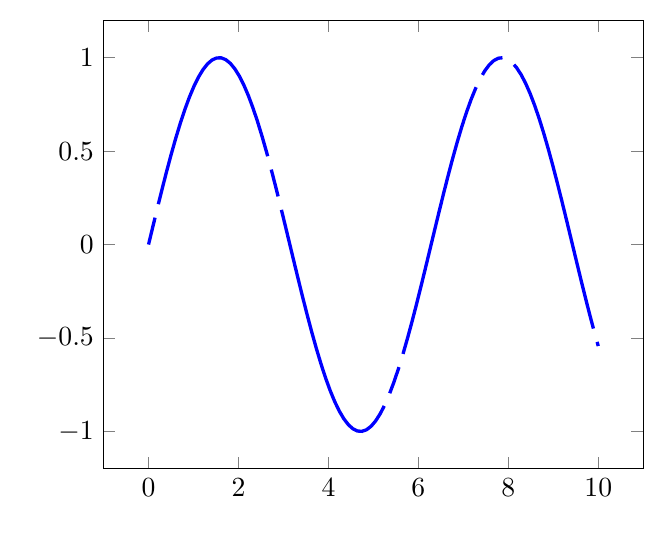
\begin{tikzpicture}
\begin{axis}
\addplot [dash pattern=on 10 off 5 on 100 off 5, domain=0:10, samples=100, very thick, blue] {sin(deg(x))};
\end{axis}
\end{tikzpicture}
\end{center}
\caption{This is generated by pgfplots!}
\end{figure}


\section{使用BibTeX 管理文献}
BibTeX 是一个使用数据库的的方式来管理参考文献程序, 用于协调LaTeX的参考文献处理。BibTeX 文件的后缀名为.bib,在你的整个研究生涯中,可以只维护这样一个.bib文件作为你的文献数据库,每一篇文献由一个唯一的ID标识,当你希望引用相关文献时,使用$\backslash$cite\{\}命令即可进行引用,并可以在你的文章末尾自动生成该篇文章引用的参考文献列表。

.bib文件中存放参考文献的条目形如:

\begin{lstlisting}[frame=single]
@inproceedings{perez2003poisson,
  title={Poisson image editing},
  author={P{\'e}rez, Patrick and Gangnet, Michel and Blake, Andrew},
  booktitle={ACM Transactions on Graphics (TOG)},
  volume={22},
  number={3},
  pages={313--318},
  year={2003},
  organization={ACM}
}
\end{lstlisting}
\vspace{1cm}

为了在\LaTeX 中使用BibTeX,必须做下面三件事情:
\begin{enumerate}
\item 设置参考文献类型:
\begin{center}
$\backslash$bibliographystyle\{plain\}
\end{center}
\item 标记引用,当你想在文档中使用引用时,插入\LaTeX 命令:
\begin{center}
$\backslash$cite\{paper--name\}
\end{center}
\item 生成参考文献列表,在文档结束前输入:
\begin{center}
$\backslash$bibliography\{bibfile\}
\end{center}
\end{enumerate}

通过Google Scholar可以轻松获取文献的BibTeX信息,如图5所示。

\begin{figure}[hbtp]
\begin{center}
\includegraphics[scale=0.5]{google_bibtex.pdf}
\end{center}
\caption{Google Scholar获取BibTeX信息}
\end{figure}

\section{使用Beamer包制作演示文稿}
Slides,即演示文稿、幻灯片的意思,用于帮助演讲者向听众传达文字、图片甚至动画和声音等信息。大部分人只接触过微软的Powerpoint,因此常用ppt代指slides,这是一种不专业的说法,Powerpoint只是一种可见即可得的slides实现方式。创建slides的方式有很多,除了使用Powerpoint,还有效果非常炫的Prezi,R语言的Slidify工具可以创建支持嵌入R程序的slides,你也可以用Javascript+HTML5自己定制基于网页的slides。这里要介绍的是\LaTeX 下的slides实现方案。

\LaTeX 上制作演示文稿(slides)的宏包非常多,有pdfscreen、prosper、context和beamer等等。目前使用的比较多的宏包是beamer,因为它的语法跟标准\LaTeX 几乎一样,通过latex和pdflatex 命令均可以编译,而且生成的slides 简洁、美观,对于科技、学术类的演示,其效果已经足够。

使用beamer创建slides的一般步骤为:
\begin{enumerate}[(1)]
\item 将\LaTeX 的文档类型从article改为beamer
\item 使用section和subsection命令组织逻辑结构
\item 使用frame命令添加独立的slide
\item 使用pdflatex命令编译两次tex文件
\end{enumerate}

下面看一个使用beamer的例子:
\begin{lstlisting}[frame=single]
\documentclass{beamer}
\usetheme{Warsaw}
\tilte{Example Presentation Created with the Beamer Package}
\author{Till Tantau}
\date{\today}

\begin{document}
\frame{\titlepage}

\section*{Outline}
\frame{\tableofcontents}

\section{Introduction}
\subsection{Overview of the Beamer Class}
\frame {
  \frametitle{\subsecname}
  \begin{itemize}
  \item<1-> Normal LaTeX class.
  \item<2-> Easy overlays.
  \item<3-> No external programs needed.
  \end{itemize}
}
\end{document}
\end{lstlisting}

使用Beamer创建slides的好处是实现了逻辑和内容的独立,使用section、subsection控制逻辑结构,使用frame创建内容。同时实现了内容和显示效果的独立,使用theme可以在不影响内容的情况下轻松的改变显示风格。

\clearpage

\section{进一步学习建议}

\begin{itemize}
\item 找一本参考资料,以备查阅,在使用中学习,不要陷入每个命令的细节中
\item 修改现成的模板,积累模板,打造自己的模板
\item Tons of information on the web
\item tex.stackexchange.com
\end{itemize}
\vspace{0.5cm}

\renewcommand\refname{参考资料}
\begin{thebibliography}{99}
\bibitem{} CTeX论坛翻译,一份不太简短的LATEX介绍
\bibitem{} 胡贤良,浙江大学数学系《数学软件》课程讲义
\bibitem{} 金秉文,如何在论文中画出漂亮的插图,http://www.zhihu.com/question/21664179
\end{thebibliography}

\end{document}
